
\documentclass{exam}

\usepackage{graphicx}
\usepackage[fleqn]{amsmath}
\usepackage{unitsdef} 
\usepackage{cancel}
\usepackage{float}
\usepackage{mdwlist}
\usepackage{booktabs}
\usepackage{cancel}
\usepackage{polynom}
\usepackage{caption}
\usepackage{fullpage}
\usepackage{enumerate}

% \newcommand{\degree}{\ensuremath{^\circ}} 
\everymath{\displaystyle}

\newunit{\inch}{in}
\newunit{\foot}{ft}
\newunit{\cemtimeter}{cm}

% \begin{figure}[H]
%   \centering
%   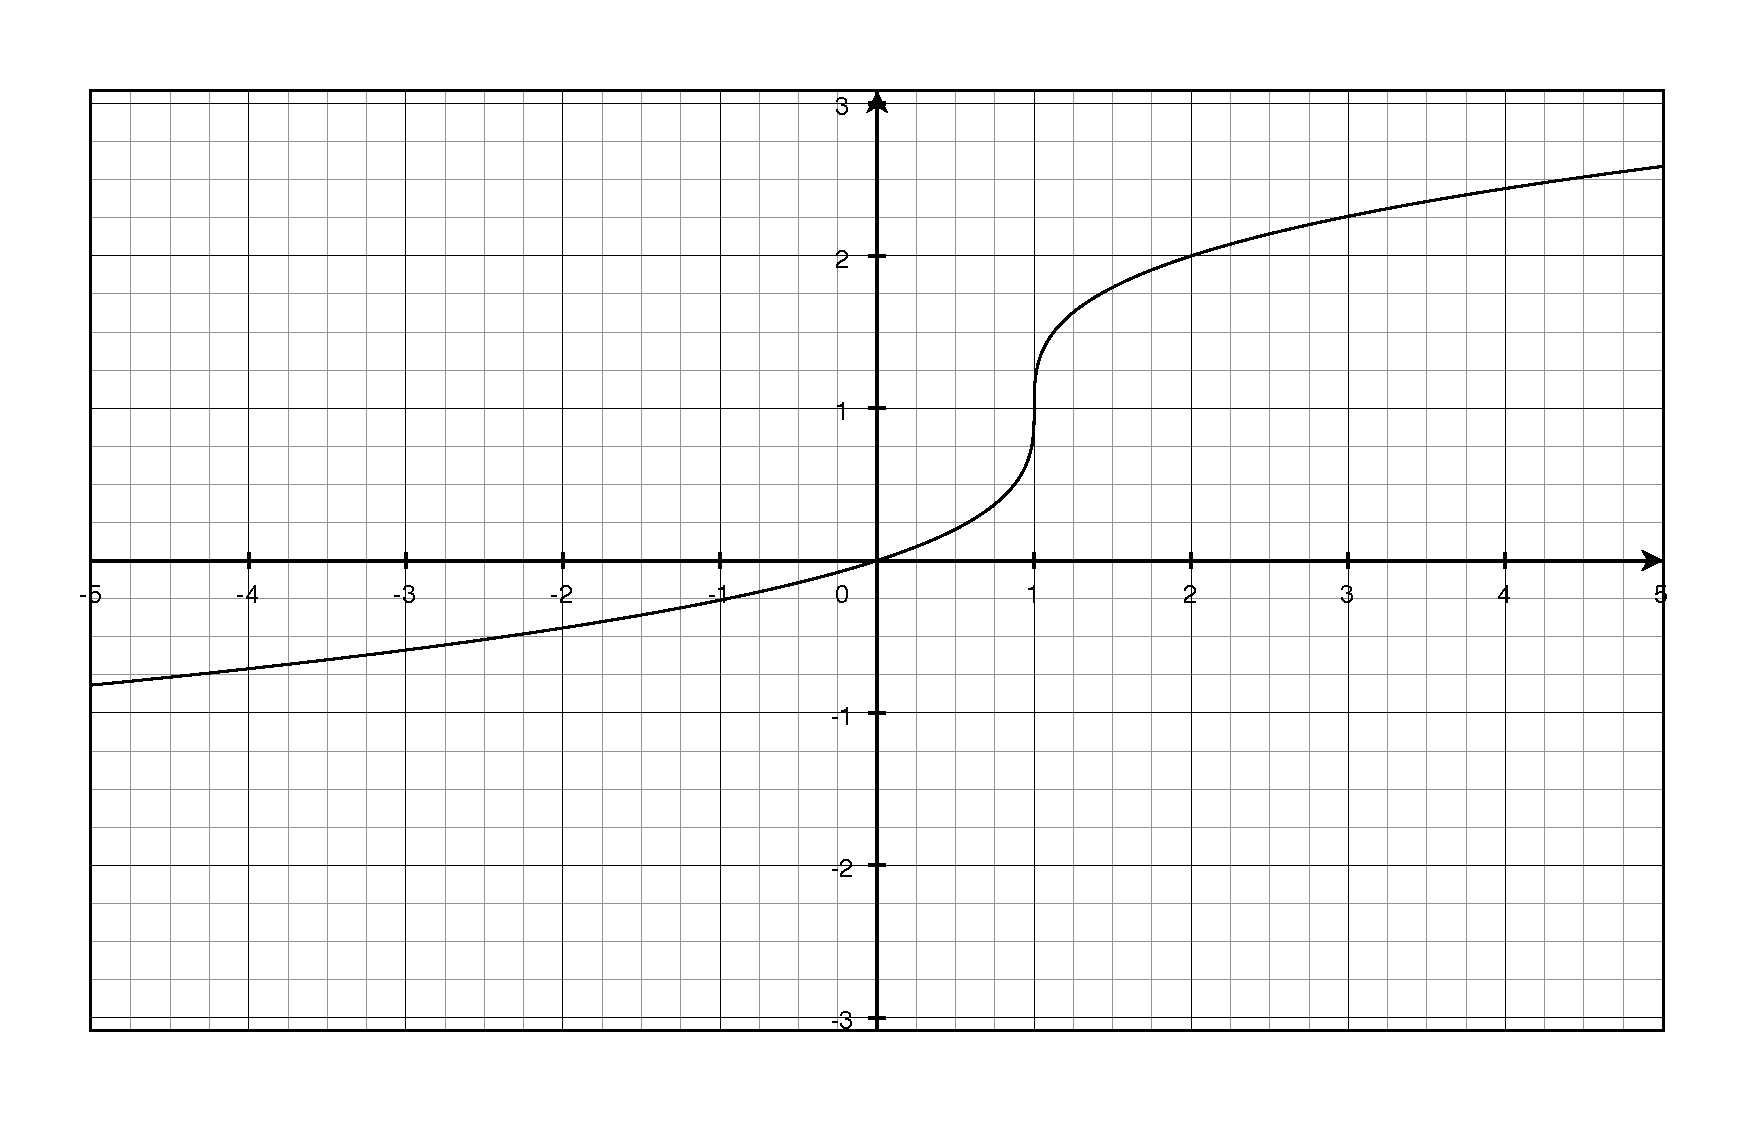
\includegraphics[scale=.3]{question7.eps}
%   \caption*{Question 7}
% \end{figure}

% \begin{tabular}{cc}
% \toprule
% period & amplitude \\
% \midrule
%   $\pi$ & $2$ \\
% \bottomrule
% \end{tabular}

\printanswers

\ifprintanswers 
\usepackage{2in1, lscape} 
\fi

\title{Math 263B \\ Homework Seven}
\date{September 6, 2012}

\begin{document}

\maketitle

\section{Homework}

\begin{itemize*}
  \item Read Section 6.1
  \item pp 302-304: 1-5, 7, 9, 11-17, 20-21, 23-24
\end{itemize*}

%% \ifprintanswers
%% \pagebreak
%% \fi

\section{Extra Credit}
page 304, problems 30 and 31

\ifprintanswers
\begin{description}
\item[30]

\begin{figure}[H]
  \centering
  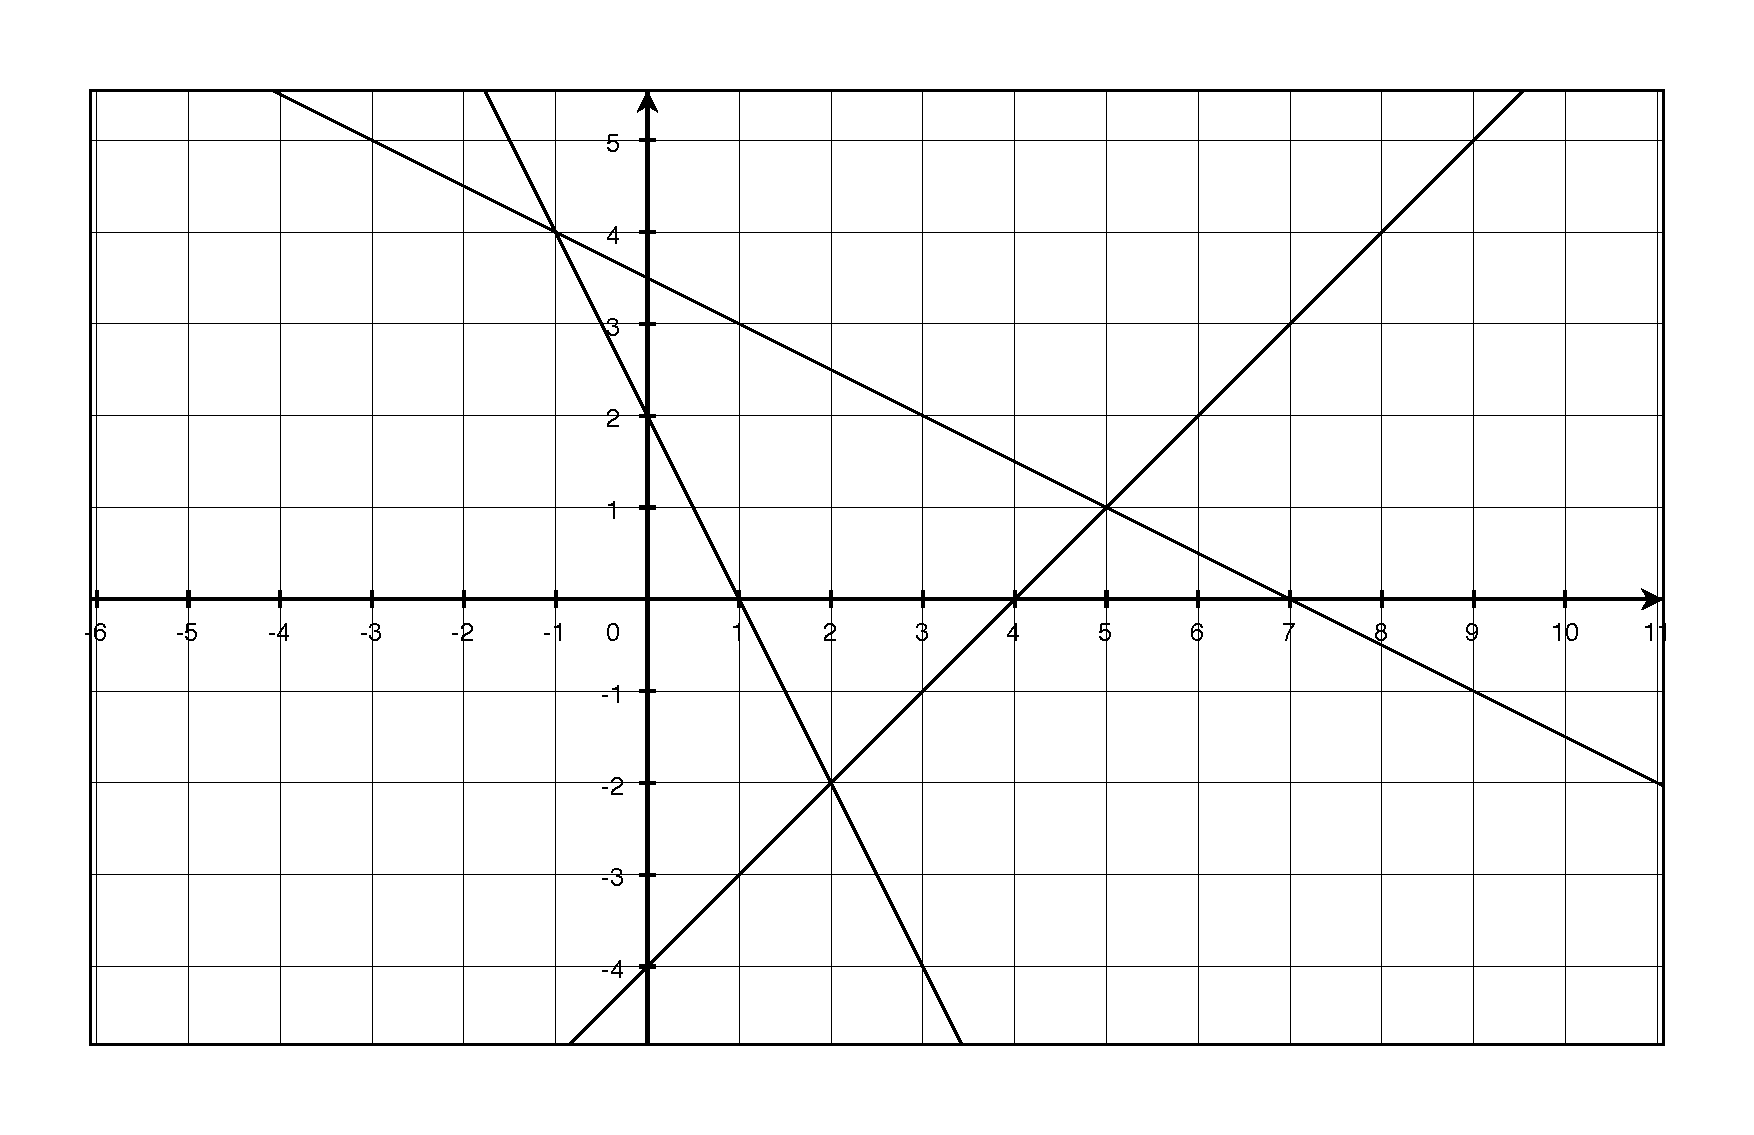
\includegraphics[scale=.3]{problem_30.eps}
  \caption*{Problem 30}
\end{figure}

The first thing to do is to find the equations of the three lines by using the points to get the slopes and
y-intercepts.  The equation are:
\begin{align*}
  y &= -\frac{1}{2} x + \frac{7}{2} \\
  y &= -2x + 2 \\
  y &= x - 4 \\
\end{align*}

There are two regions in the area.  The first region goes from $-1$ to 2:
\[
  \int_{-1}^2 \left[ -\frac{1}{2} x + \frac{7}{2} - (-2x + 2) \right] \, \mathrm{d}x = \frac{27}{4}
\]

The second region goes from 2 to 5:
\[
  \int_2^5 \left[ -\frac{1}{2} x + \frac{7}{2} - (x - 4) \right] \, \mathrm{d}x = \frac{27}{4}
\]

The total area is the sum of these two areas:
\[
  A = 2 \cdot \frac{27}{4} = \frac{27}{2}
\]

\item[31]
\begin{figure}[H]
  \centering
  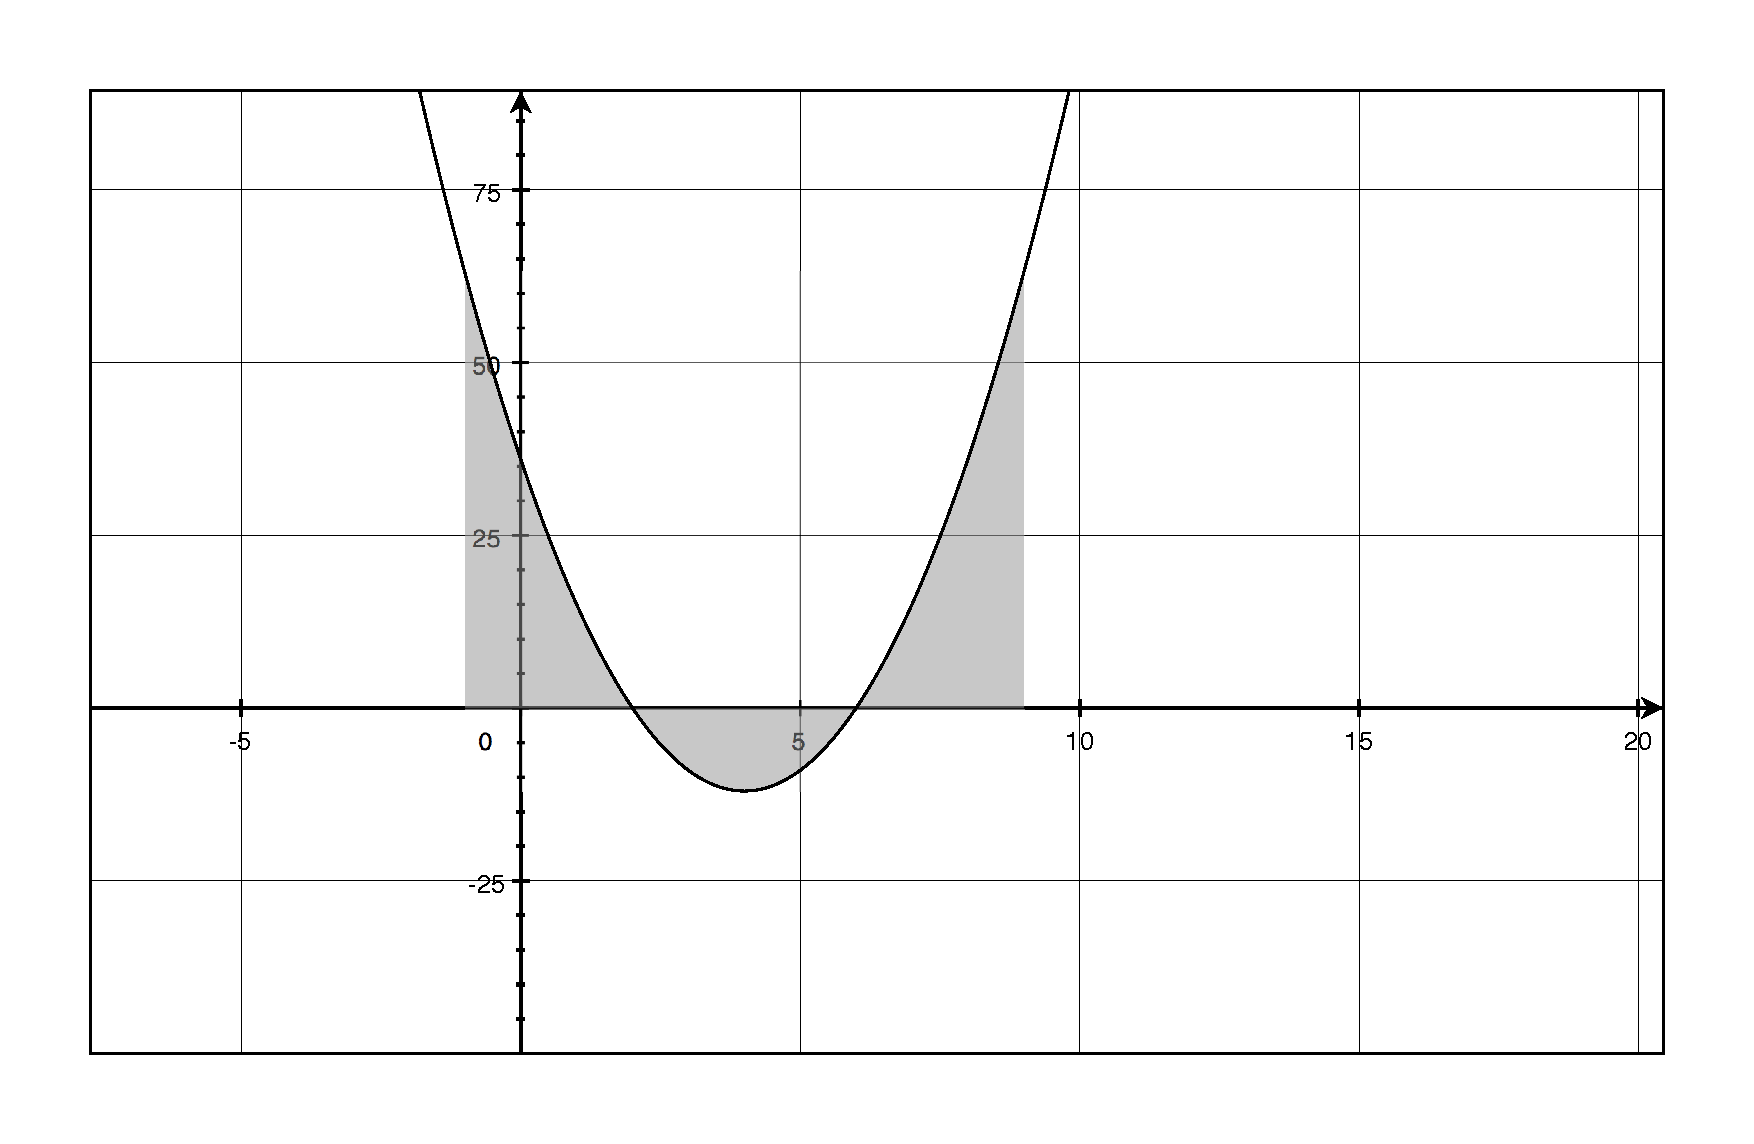
\includegraphics[scale=.3]{problem_31.eps}
  \caption*{Problem 31}
\end{figure}

The displacement is the integral of the velocity:
\[
  displacement = \int_{-1}^9 (3t^2 - 24t + 36) \, \mathrm{d}t = 130
\]

The object is moving backwards between 2 and 6, so the total distance traveled is:
\begin{align*}
  distance &= \int_{-1}^2 (3t^2 - 24t + 36) \, \mathrm{d}t - \int_2^6 (3t^2 - 24t + 36) \, \mathrm{d}t \\
  &+ \int_6^9 (3t^2 - 24t + 36) \, \mathrm{d}t \\
  &= 194 \\
\end{align*}

\uplevel{\section{Section 6.1}}

\item[1]
\[
\int_{-1}^2 (x^2 + 1) \, \mathrm{d}x = 6
\]

\item[2]
\[
\int_{-1}^2 (x^3 - x + 2) \, \mathrm{d}x = \frac{33}{4}
\]

\item[3]
\[
\int_{-1}^2 [ x^2 + 2 - (-x) ] \, \mathrm{d}x = \int_{-1}^2 ( x^2 + x + 2) \, \mathrm{d}x = \frac{40}{3}
\]

\item[4]
\[
  - \int_{-3}^1 (x^2 + 2x - 3) \, \mathrm{d}x = \frac{32}{3}
\]

\item[5]
Find the points of intersection:
\begin{align*}
  2 - x^2 &= x \\
  x^2 + x - 2 &= 0 \\
  (x + 2)(x - 1) &= 0 \\
  x &= \{-2, 1\} \\
\end{align*}

Find the area:
\[
  \int_{-2}^1 (2 - x^2 - x) \, \mathrm{d}x = \frac{9}{2}
\]

\item[7]
Find the points where the curve crosses the x-axis:
\begin{align*}
  x^3 - x^2 - 6x &= 0 \\
  x &= \{-2, 0, 3\} \\
\end{align*}

Find the area:
\[
  \int_{-2}^0 (x^3 - x^2 - 6x) \, \mathrm{d}x - \int_0^3 (x^3 - x^2 - 6x) \, \mathrm{d}x = \frac{253}{12}
\]

\item[9]
Find the points where the curve crosses the y-axis:
\begin{align*}
  y + 1 &= 3 - y^2 \\
  y &= \{-2, 1\} \\
\end{align*}

Find the area:
\[
  \int_{-2}^1 (3 - y^2) - (y + 1) \, \mathrm{d}y = \int_{-2}^1 (-y^2 - y + 2) \, \mathrm{d}y = \frac{9}{2}
\]

\item[11]
\[
  \int_0^3 \left(3 - \frac{1}{3} x^2 \right) \, \mathrm{d}x = 6
\]

\begin{figure}[H]
  \centering
  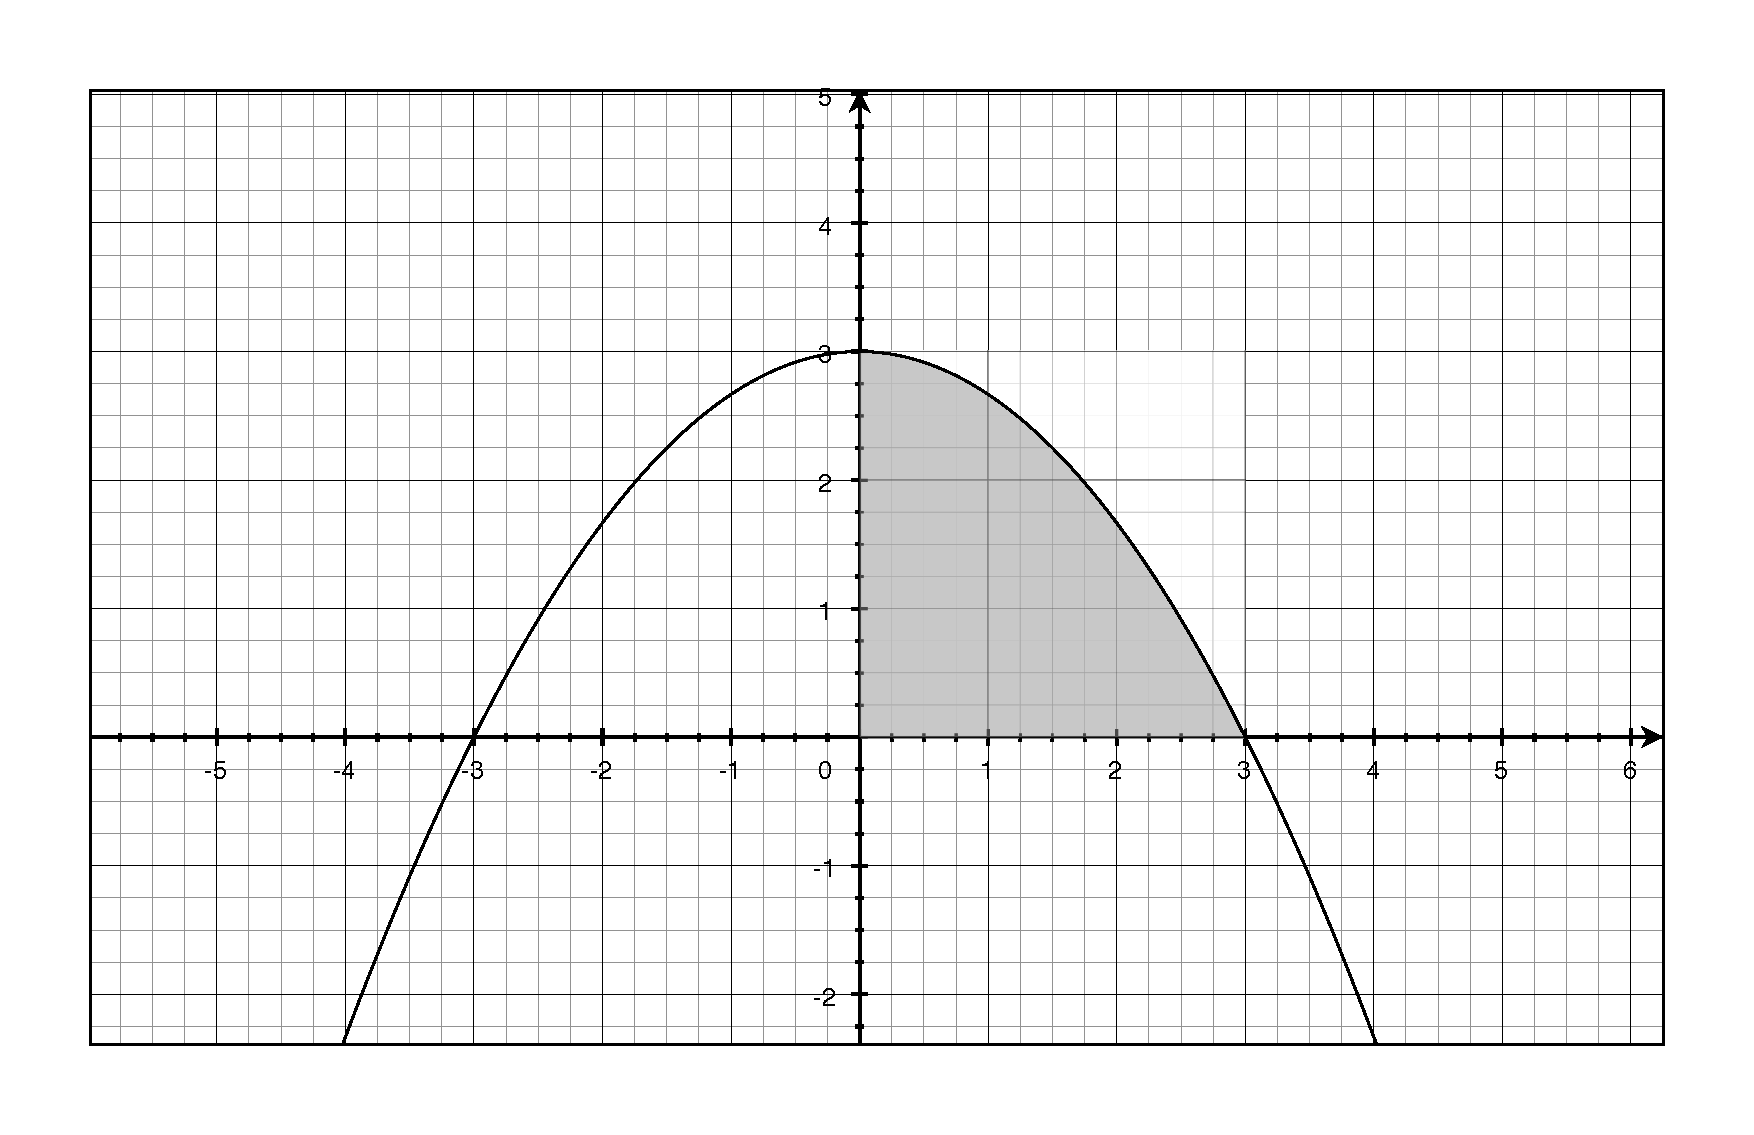
\includegraphics[scale=.3]{problem_11.eps}
  \caption*{Problem 11}
\end{figure}

\item[12]
\[
  \int_0^3 \left(5x - x^2 \right) \, \mathrm{d}x = \frac{34}{3}
\] 

\begin{figure}[H]
  \centering
  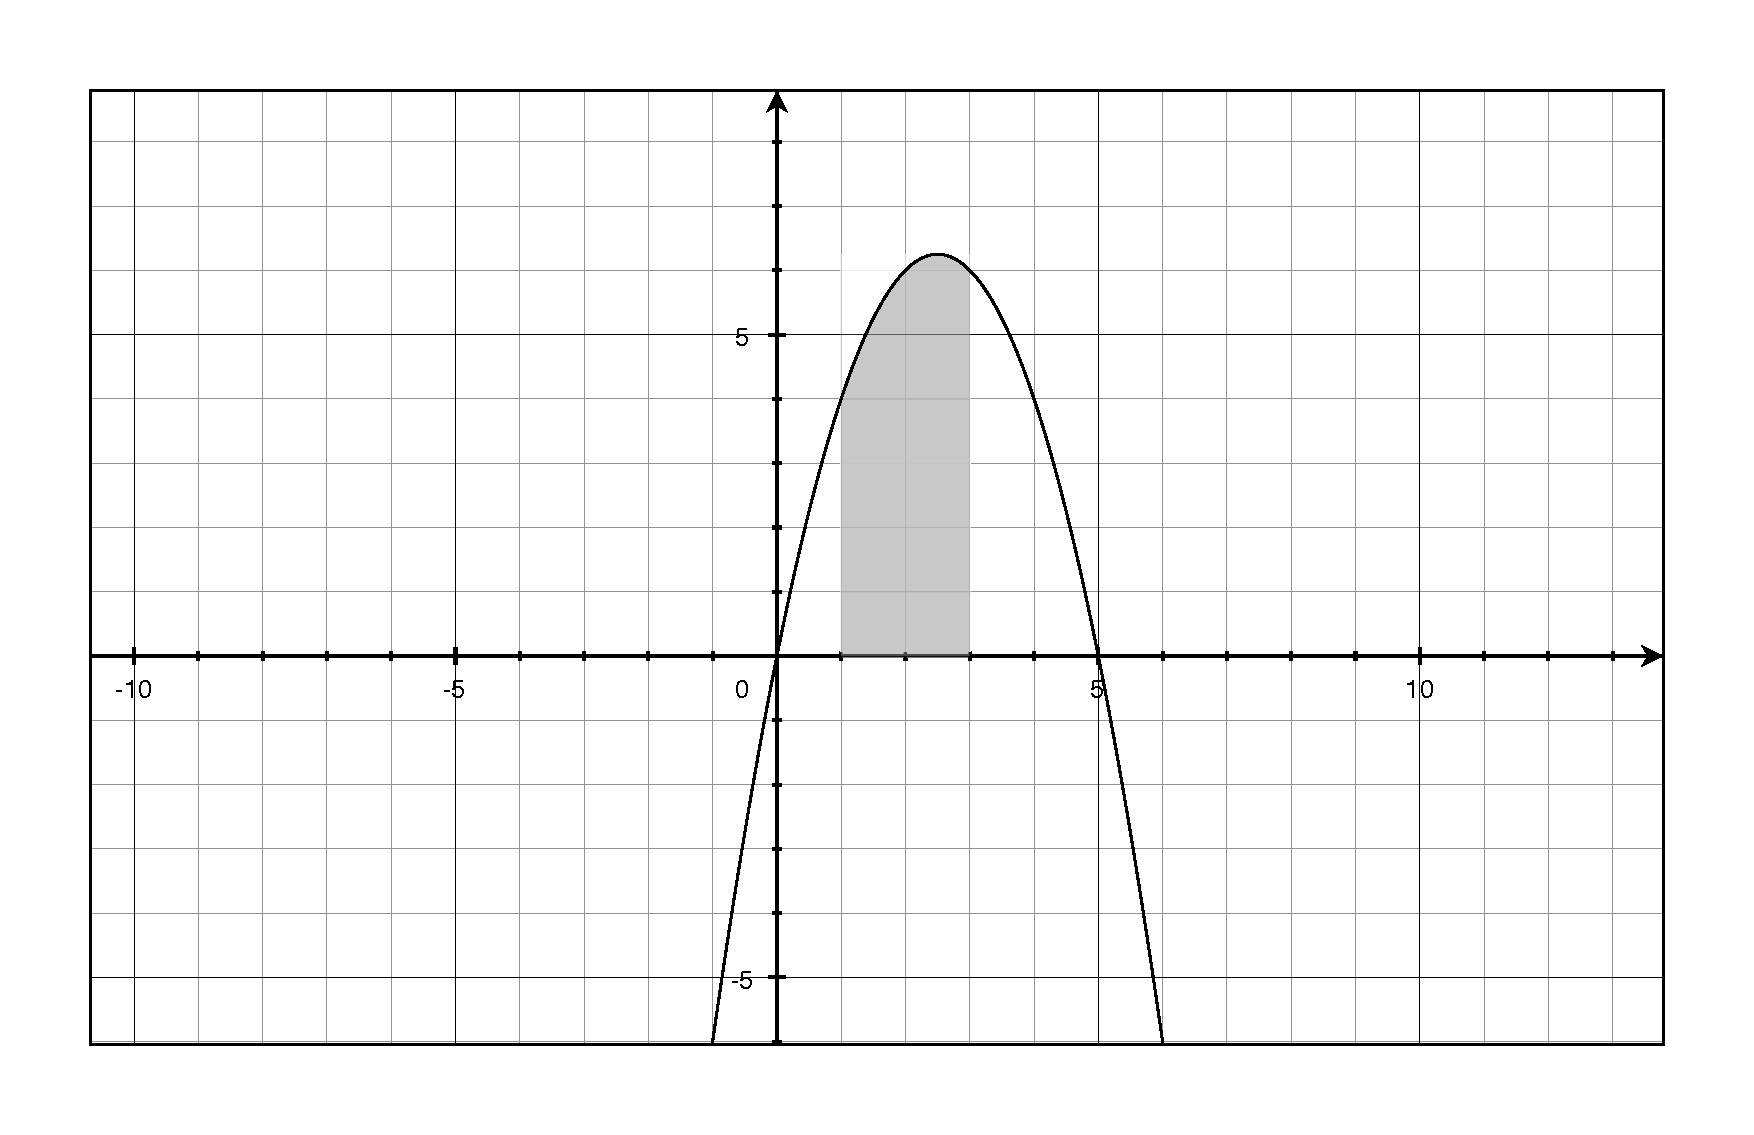
\includegraphics[scale=.3]{problem_12.eps}
  \caption*{Problem 12}
\end{figure}

\item[13]
\[
  - \int_0^3 (x - 4)(x + 2) \, \mathrm{d}x = - \int_0^3 (x^2 - 2x - 8) \, \mathrm{d}x = 24
\] 

\begin{figure}[H]
  \centering
  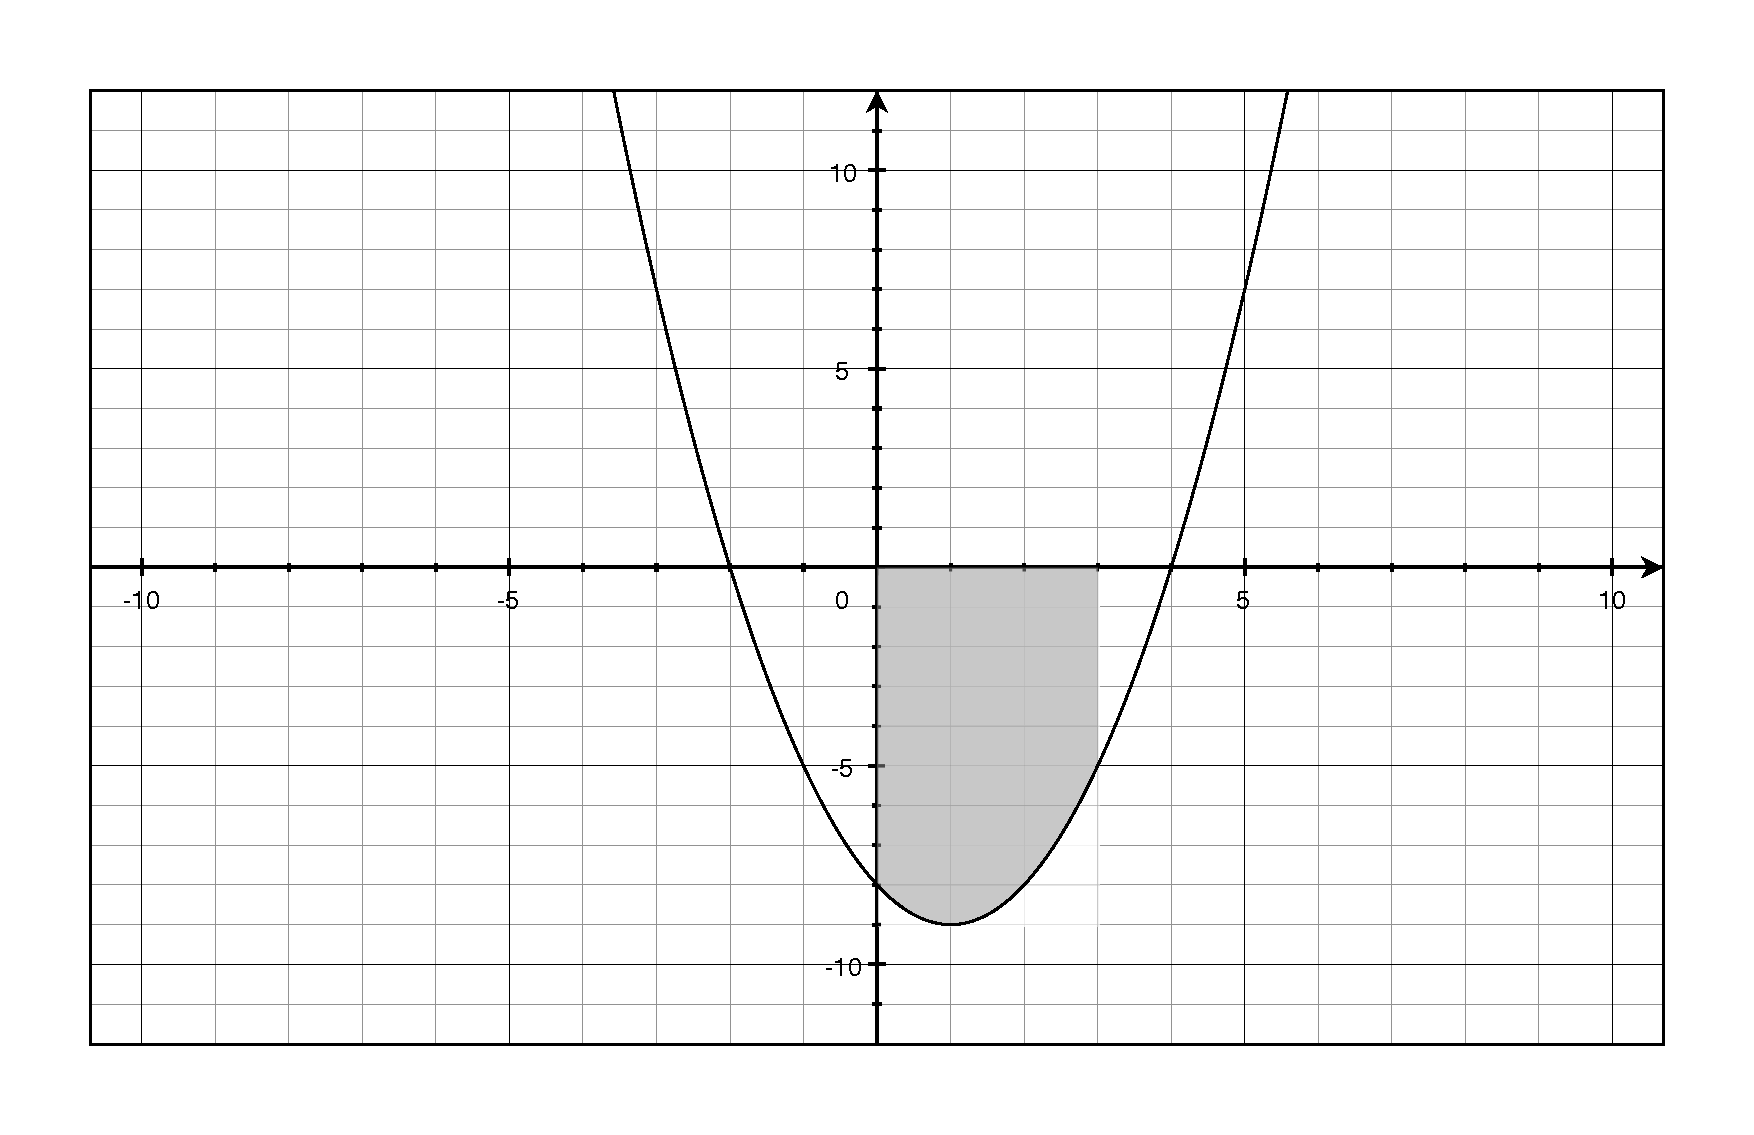
\includegraphics[scale=.3]{problem_13.eps}
  \caption*{Problem 13}
\end{figure}

\item[14]
\[
  - \int_{-1}^4 (x^2 - 4x - 5) \, \mathrm{d}x = \frac{100}{3}
\] 

\begin{figure}[H]
  \centering
  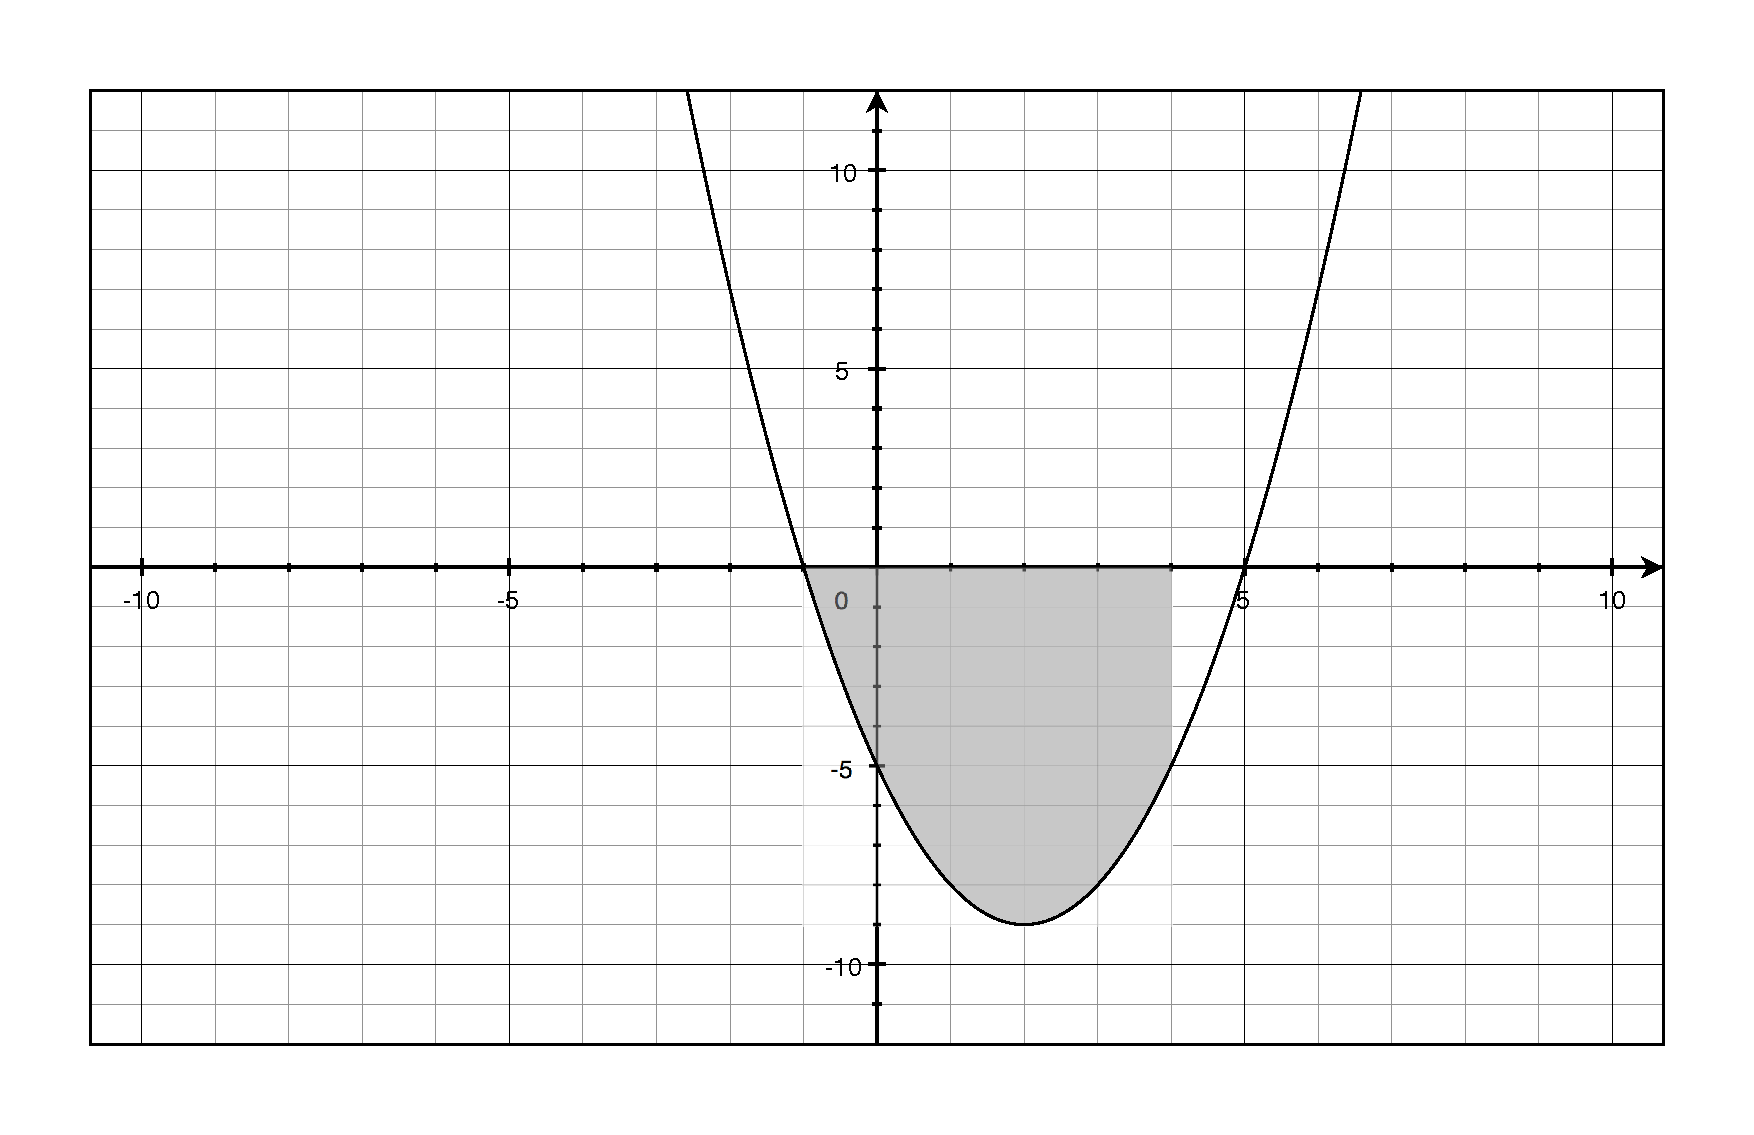
\includegraphics[scale=.3]{problem_14.eps}
  \caption*{Problem 14}
\end{figure}

\item[15]
\[
  - \int_0^2 \frac{1}{4} (x^2 - 7) \, \mathrm{d}x = \frac{17}{6}
\] 

\begin{figure}[H]
  \centering
  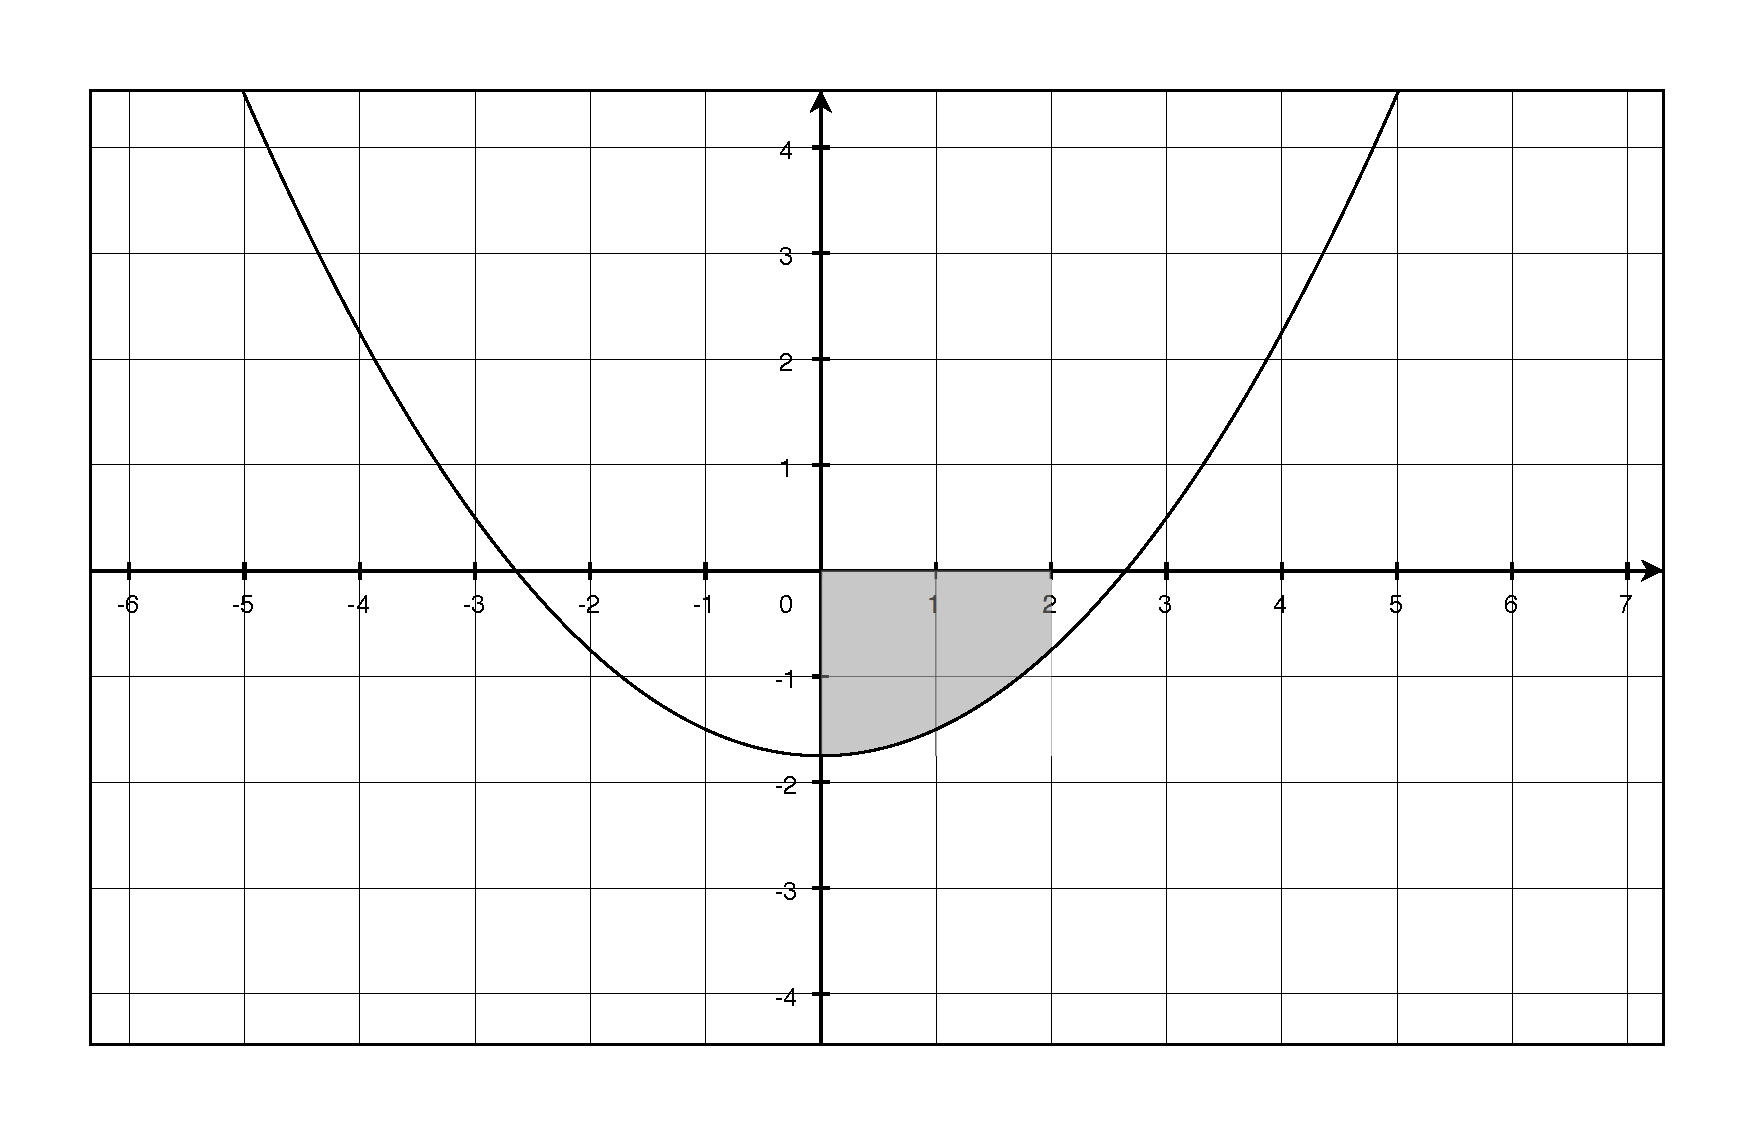
\includegraphics[scale=.3]{problem_15.eps}
  \caption*{Problem 15}
\end{figure}

\item[16]
\[
  2 \int_0^3 x^3 \, \mathrm{d}x = \frac{81}{2}
\] 

\begin{figure}[H]
  \centering
  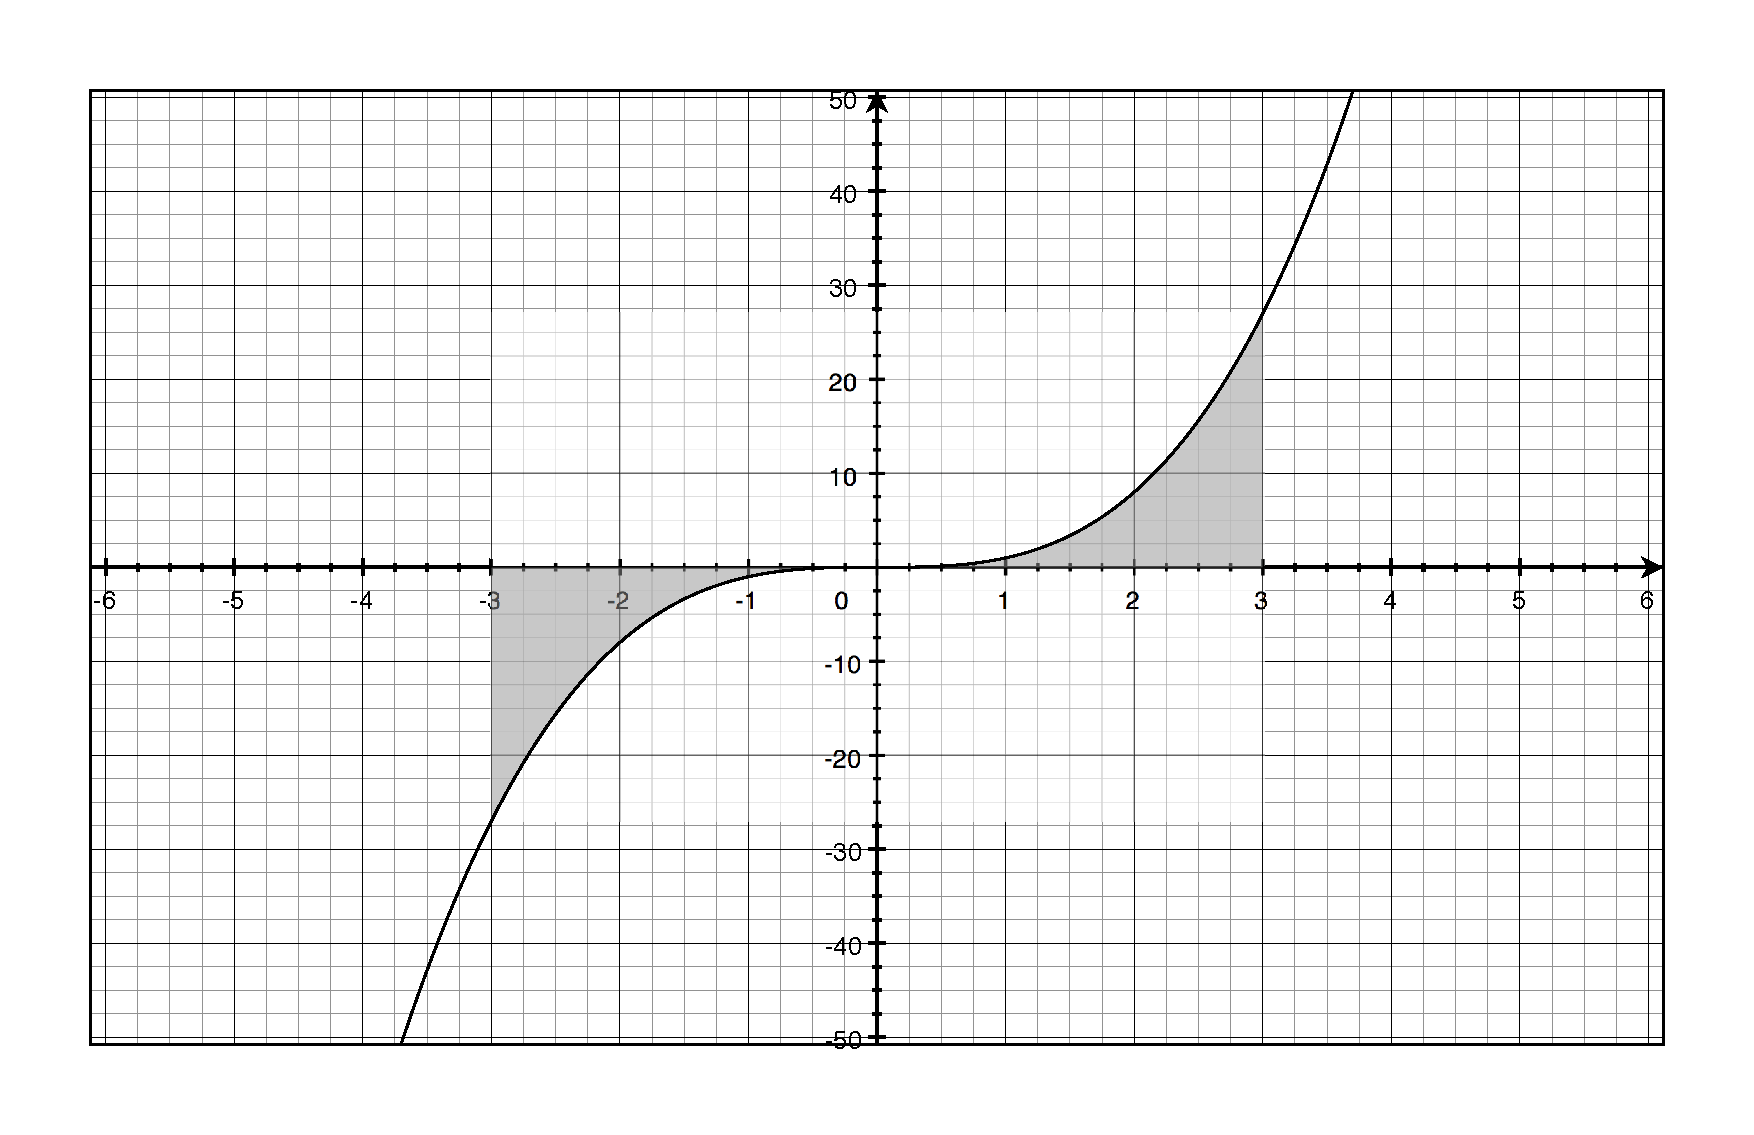
\includegraphics[scale=.3]{problem_16.eps}
  \caption*{Problem 16}
\end{figure}

\item[17]
\[
  2 \int_0^2 x^{1/3} \, \mathrm{d}x = 3 \sqrt[3]{2}
\] 

\begin{figure}[H]
  \centering
  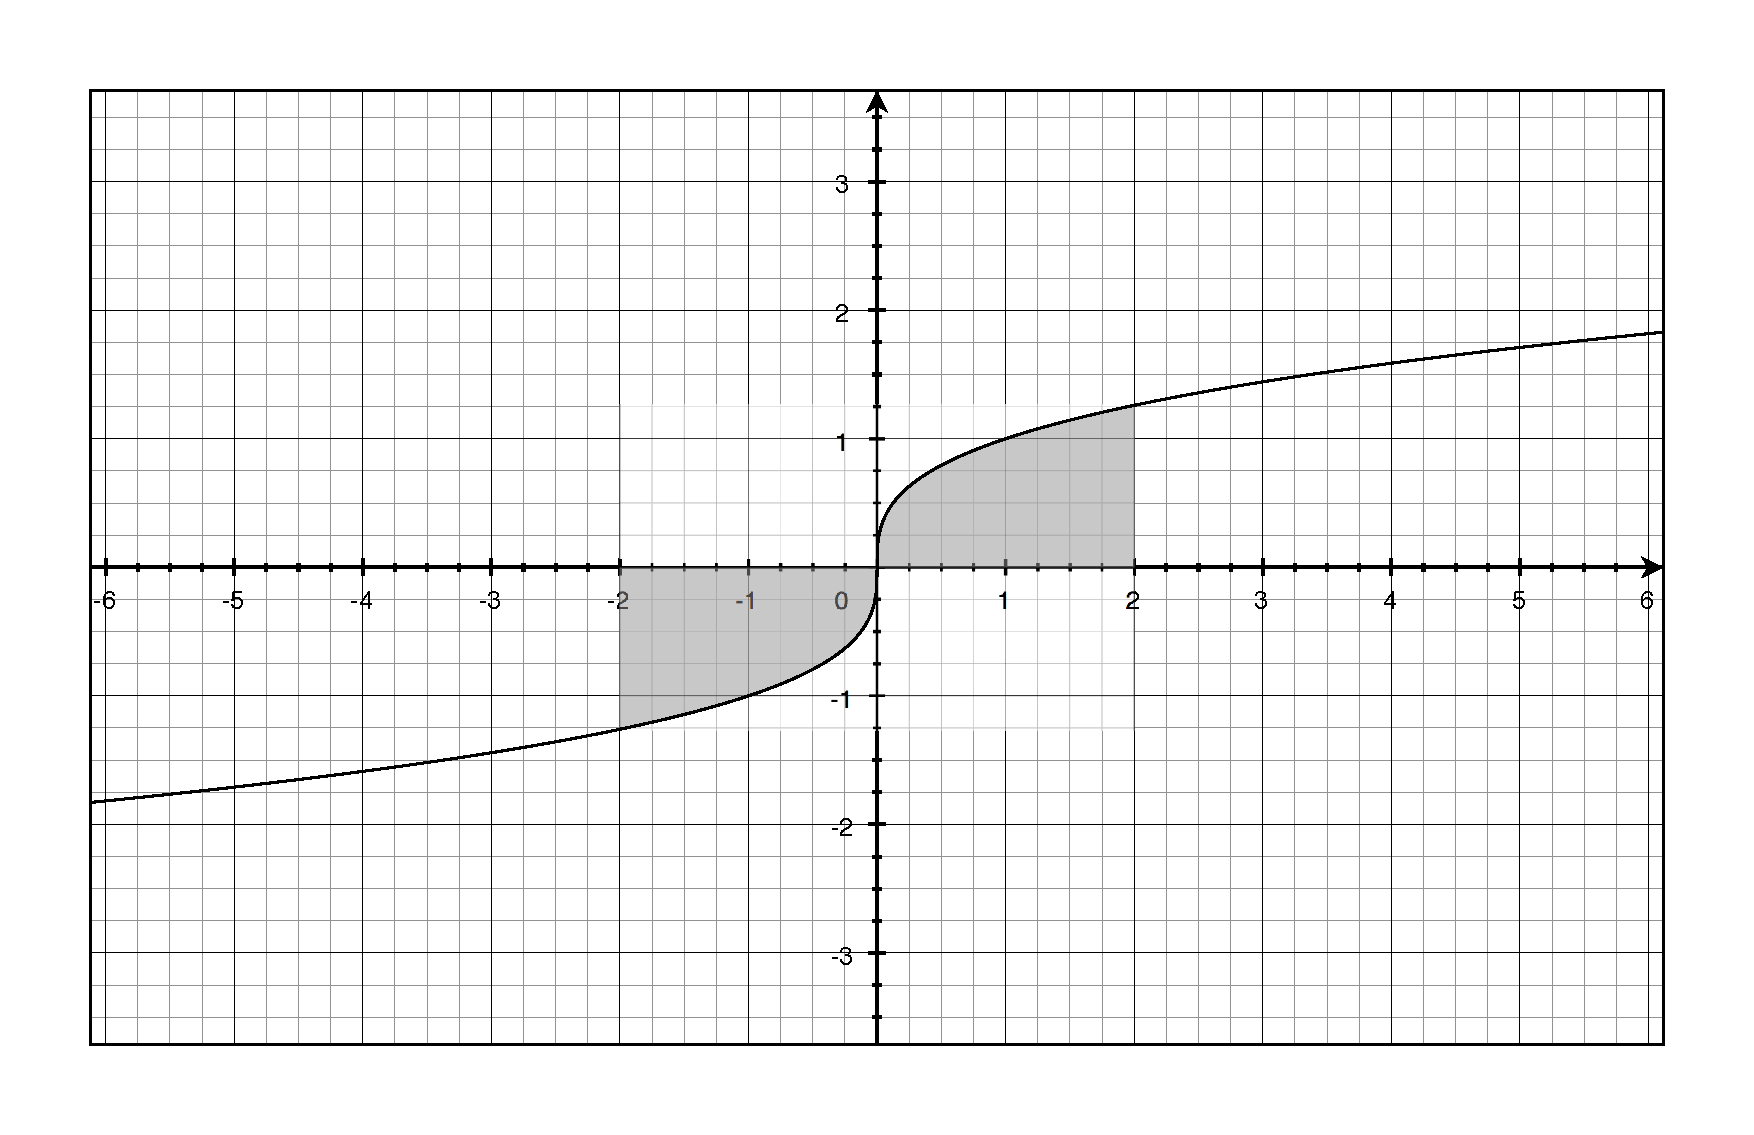
\includegraphics[scale=.3]{problem_17.eps}
  \caption*{Problem 17}
\end{figure}

\item[20]
Find points of intersection:
\begin{align*}
  3 \sqrt{x} &= x - 4 \\
  9x &= x^2 - 8x + 16 \\
  x &= 16 \\
\end{align*}

$x = 1$ is an extraneous solution which doesn't actuall work.  $y = 3\sqrt{x}$ is only defined for $x \geq 0$, so 0 is the lower bound for the integral.

Find area
\[
  \int_0^{16} [ 3x^{1/2} - (x - 4)] \, \mathrm{d}x = 64 \\
\] 

\begin{figure}[H]
  \centering
  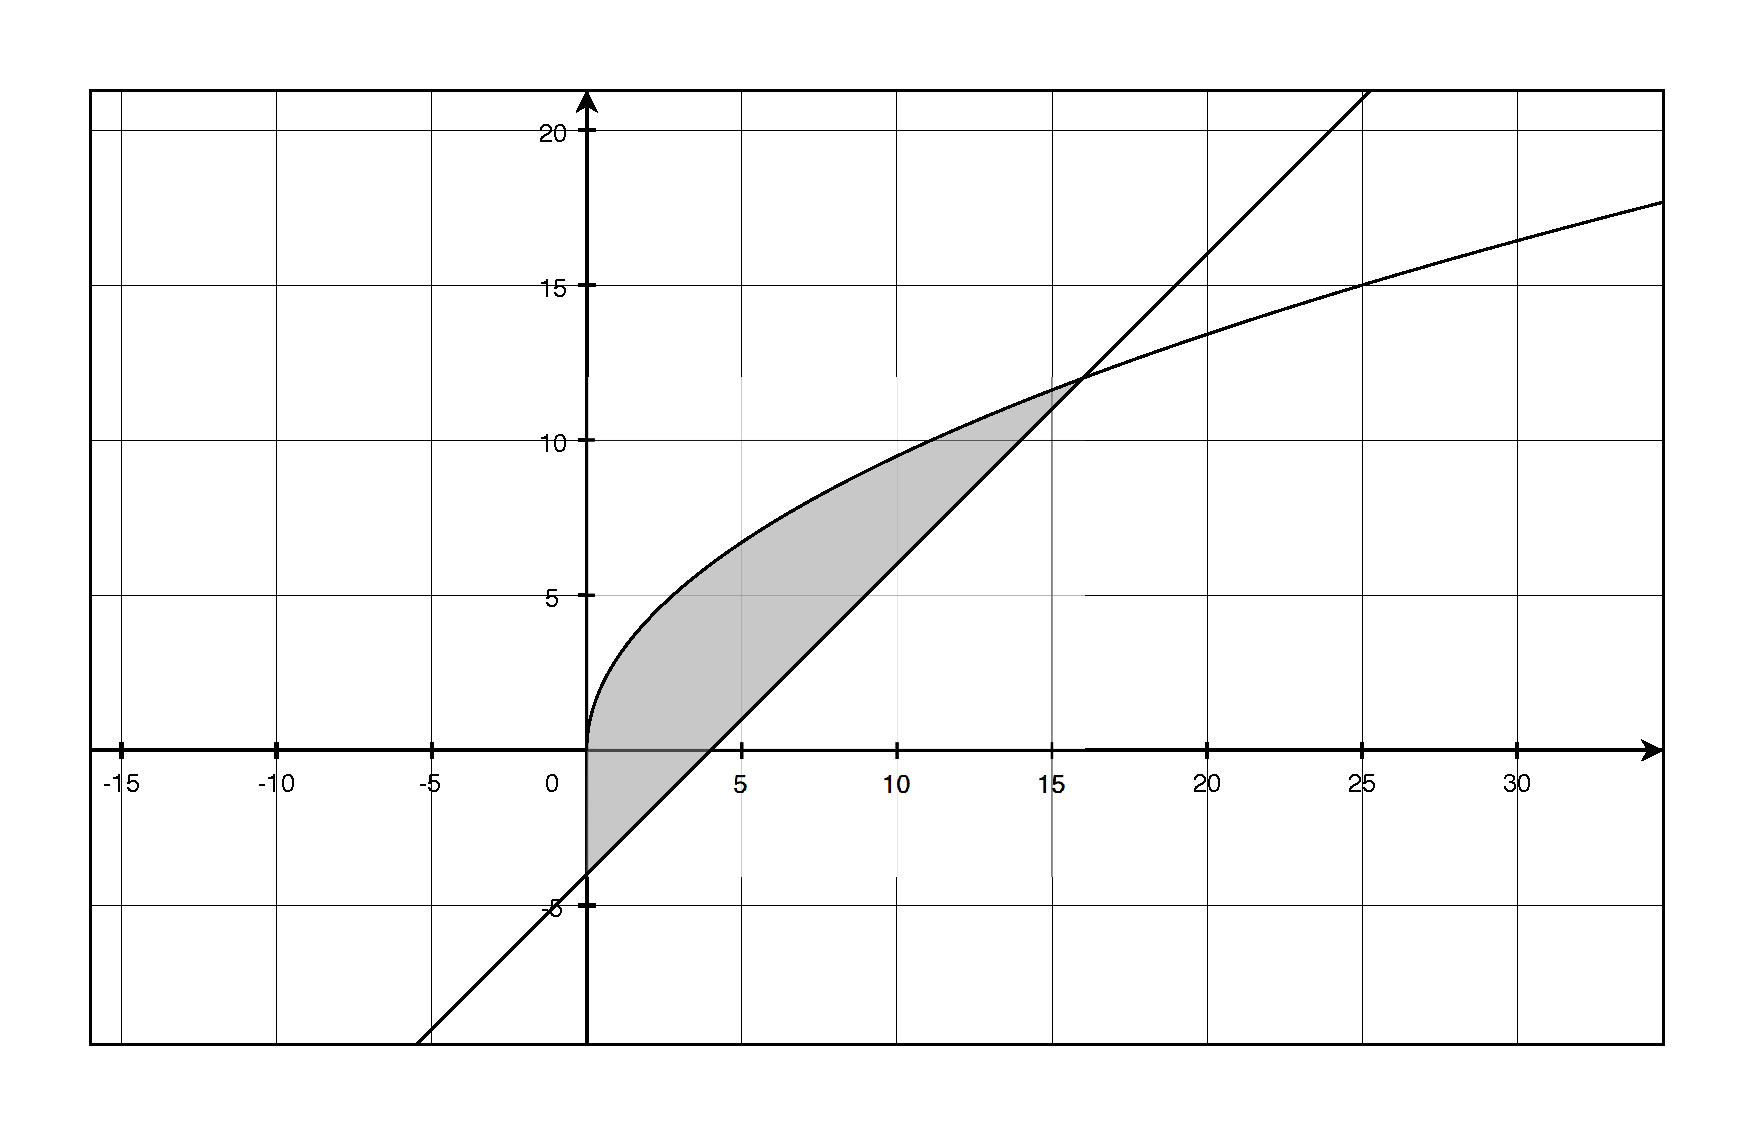
\includegraphics[scale=.3]{problem_20.eps}
  \caption*{Problem 20}
\end{figure}

\item[21]
\begin{figure}[H]
  \centering
  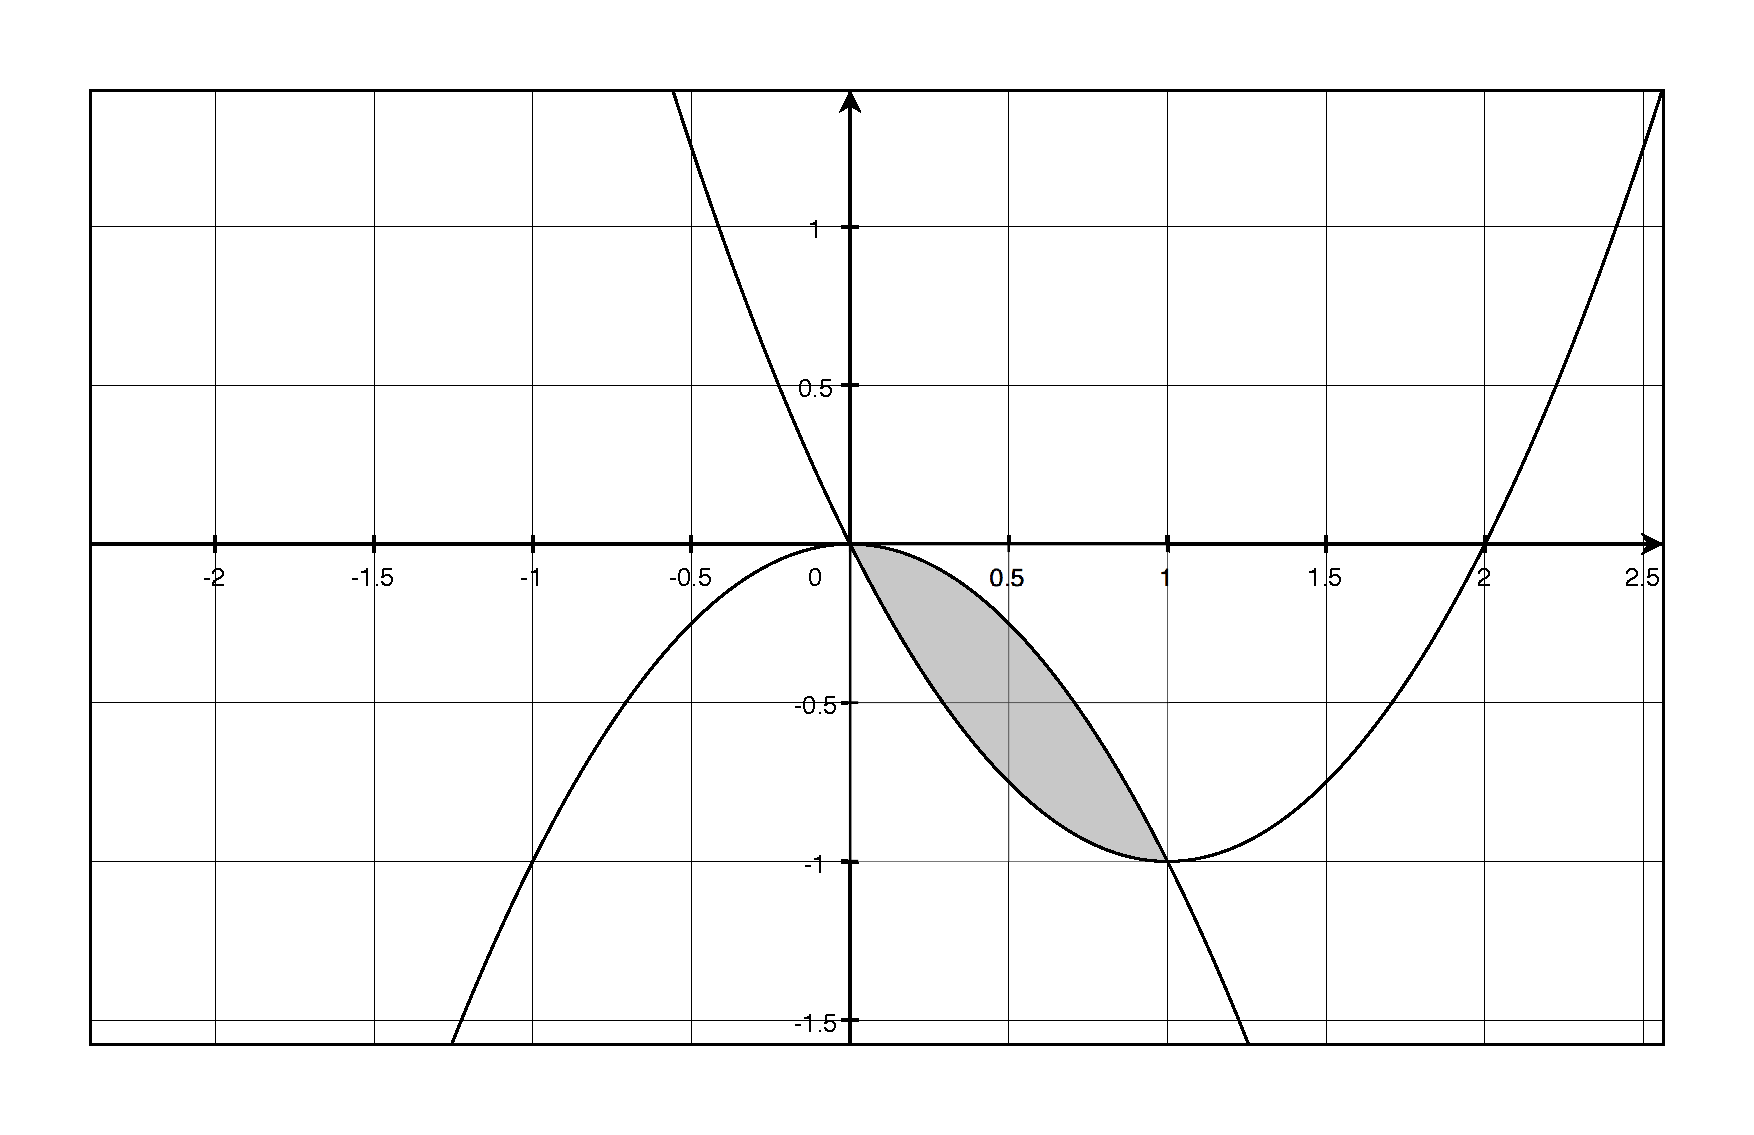
\includegraphics[scale=.3]{problem_21.eps}
  \caption*{Problem 21}
\end{figure}

Find points of intersection:
\begin{align*}
  x^2 - 2x &= -x^2 \\
  x &= \{0, 1\} \\
\end{align*}

Find area
\[
  \int_0^1 [ (x^2 - 2x) - x^2 ] \, \mathrm{d}x = \int_0^1 (2x^2 - 2x) \, \mathrm{d}x = \frac{1}{3}
\] 

\item[23]
Find points of intersection:
\begin{align*}
  8y - y^2 &= 0 \\
  y &= \{0, 8\} \\
\end{align*}

Find area
\[
  \int_0^8 (8y - y^2) \, \mathrm{d}y = \frac{256}{3}
\] 

\begin{figure}[H]
  \centering
  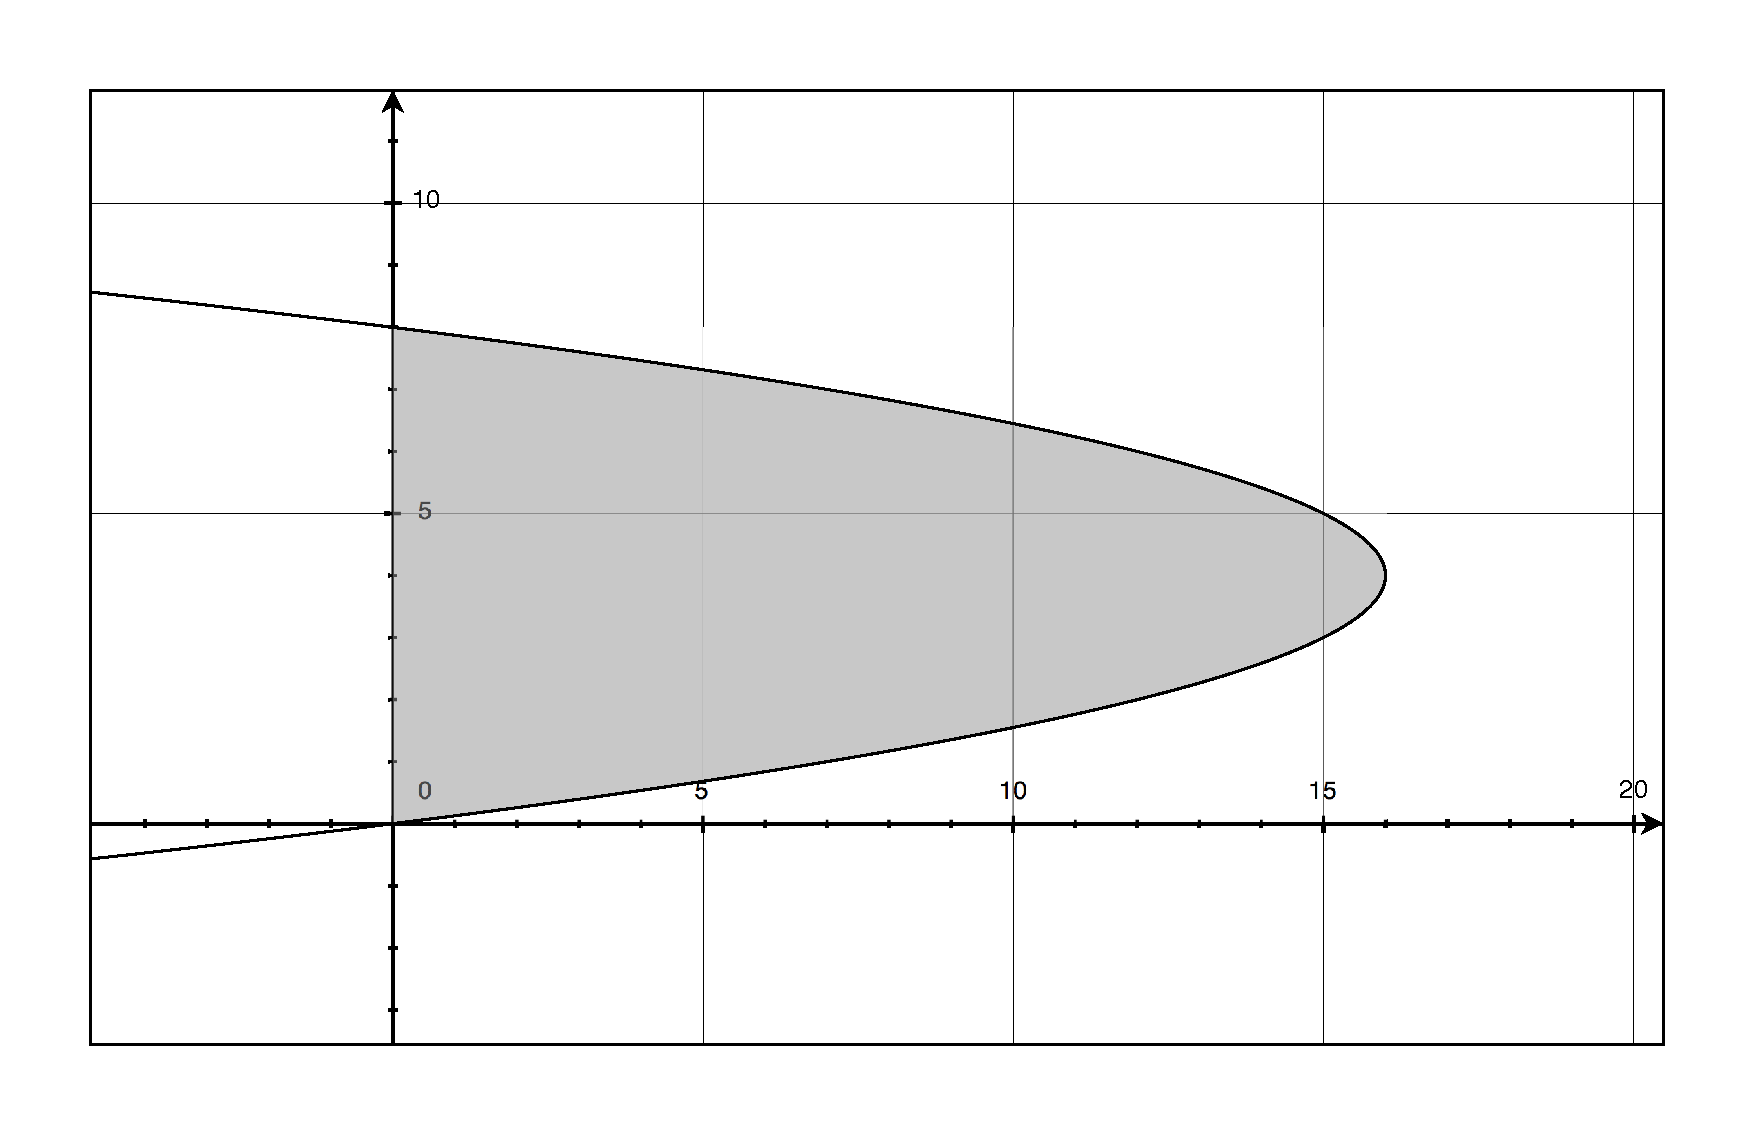
\includegraphics[scale=.3]{problem_23.eps}
  \caption*{Problem 23}
\end{figure}

\item[24]
\[
  \int_{-1}^3 [(3 - y)(y+1) ] \, \mathrm{d}y = \int_{-1}^3 (-y^2 + 2y + 3) \, \mathrm{d}y = \frac{32}{3}
\] 

\begin{figure}[H]
  \centering
  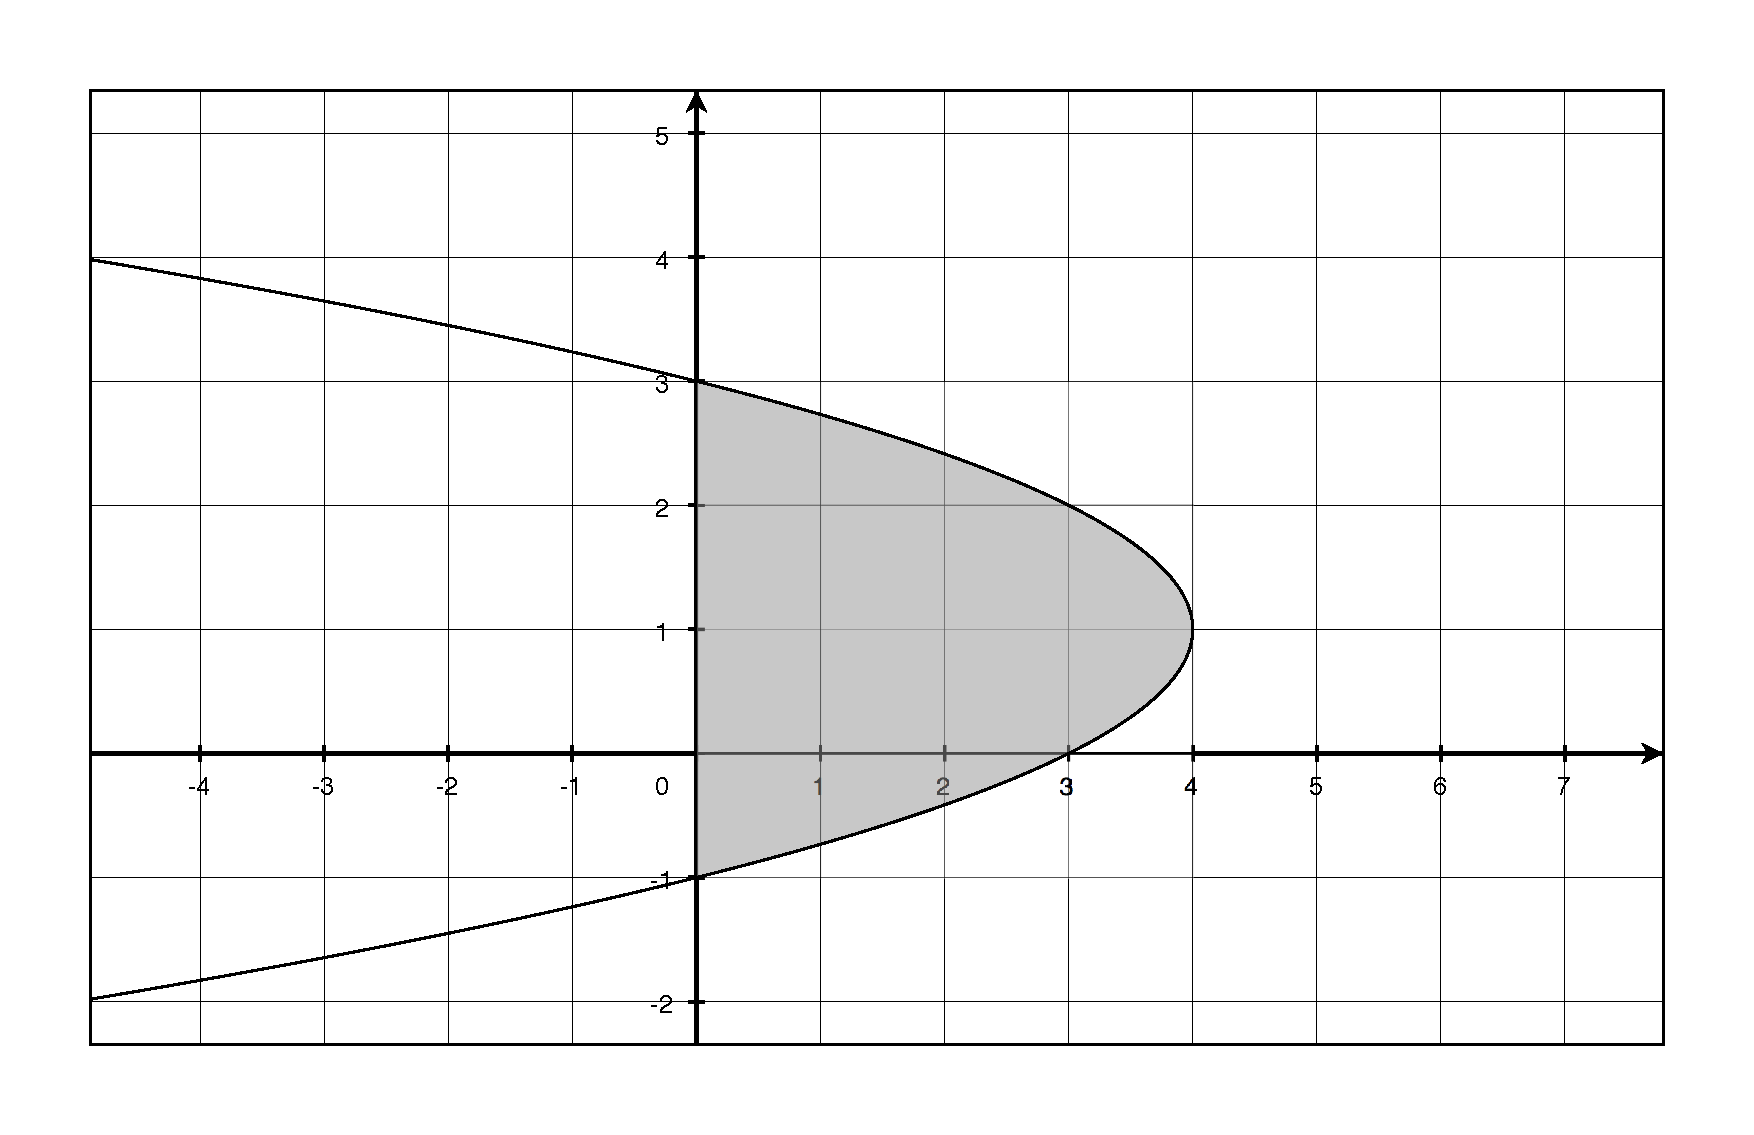
\includegraphics[scale=.3]{problem_24.eps}
  \caption*{Problem 24}
\end{figure}


\end{description}

\else

\vspace{10 cm}

%% The most effective way to restrict democracy is to transfer decision-making from the public arena to unaccountable
%% institutions: kings and princes, priestly castes, military juntas, party dictatorships, or modern corporations.

%% \hspace{0.5 cm} --Noam Chomsky

%% {\em Some writers have so confounded society with government, as to leave little or no distinction between them; whereas
%%   they are not only different, but have different origins. Society is produced by our wants, and government by our
%%   wickedness; the former promotes our happiness POSITIVELY by uniting our affections, the latter NEGATIVELY by
%%   restraining our vices. The one encourages intercourse, the other creates distinctions. The first a patron, the last a
%%   punisher.} --Thomas Paine

{\em Peace cannot be kept by force.  It can only be achieved by understanding.}

\vspace{.2 cm}

\hspace{1 cm} --Albert Einstein

\fi

\end{document}

